\subsection{Потенциальный код без возврата к нулю (NRZ)}
Для определения верхней границы частот необходимо найти наиболее высокочастотную составляющую спектра в передаваемом сообщении, которая в NRZ образуется при передаче чередующихся значений 0 и 1, при этом период гармонического сигнала (синусоиды), используемого для передачи прямоугольных сигналов 0 и 1, будет равен удвоенной длительности битового интервала $\tau: T = 2\tau$, где $\tau$ определяется как величина, образная значению пропускной способности канала $C: \tau = \frac{1}{C}$. Отсюда верхняя граница частот будет равна \[f_{\text{в}} = \frac{1}{T} = \frac{C}{2}\]

То есть, при пропускной способности канала связи $C = 10 \, \text{Мбит/с}$ частота основной гармоники равна $f_{\text{в}} = \frac{10 \cdot 10^3}{2} = 5 \, \text{МГц}$, а битовый интервал $\tau = 100 \, \text{нс}$.

В общем случае, при кодировании любого сообщения с помощью метода NRZ наибольшая (верхняя) частота достигается при передаче чередующихся значений 0 и 1, а наименьшая (нижняя) - при передаче длинных (в пределе - бесконечных) последовательностей нулей и единиц, что делает нижнюю границу частот близкой и в пределе равной нулю: $f_{\text{н}} = 0$. Следовательно, в предельном случае спектр: $S = f_{\text{в}} - f_{\text{н}} = f_{\text{в}} = \frac{C}{2}$.

С другой стороны, при передаче конкретного сообщения нижняя частота всегда больше нуля и зависит от максимальной длины последовательностей нулей или единиц. В этом случае для расчёта нижней границы чапстот необходимо в коде передаваемого сообщения найти \textit{наиболее длинную последовательность 1 или 0}. В исходном сообщении, закодированном по методу NRZ, представленному на рисунке 1, низкочастотная составляющая образуется при передаче 6 последовательных нулей. Период синусоидального сигнала при передаче таких последовательностей равен 12 битовым интервалам и нижняя граница частот соответственно будет равна: $f_{\text{н}} = \frac{1}{12\tau} = \frac{C}{12}$. Тогда \textbf{спектр} при передаче данного сообщения кодом NRZ равен
\[
	S =  f_{\text{в}} - f_{\text{н}} = \frac{C}{2} - \frac{C}{12} = \frac{5C}{12} = 4.167 \, \text{МГц}
\]

Среднее значение частоты передаваемого сообщения находится в интервале $(f_{\text{н}};f_{\text{в}})$ и показывает, какие частоты (низкие или высокие) превалируют в спектре передаваемого сигнала.

Для оценки среднего значения частоты передаваемого сообщения можно для каждого битового интервала определить соответствующую частоту сигнала, просуммировать их и разделить на количество битовых интервалов. В нашем случае: частота основной гармоники $f_0 = \frac{C}{2}$ соответствует трём битовым интервалам, частота вдвое меньшая, т.е. $\frac{f_0}{2}$, соответствует также трём битовым интервалам, частота $\frac{f_0}{3}$ - четырём битовым интервалам, $\frac{f_0}{5}$ - одному битовому интервалу, и $\frac{f_0}{6}$ - одному битовому интервалу.

Тогда средняя частота рассматриваемого сообщения
\[
	f_{\text{ср}} = \left(3f_0+3\frac{f_0}{2}+4\frac{f_0}{3}+\frac{f_0}{5}+\frac{f_0}{6}\right)/ 12 = \frac{31f_0}{60} = \frac{31 \cdot 5}{60} \approx 2.583 \, \text{МГц}
\]

Поскольку середине спектра рассматриваемого сообщения соответствует частота
\[
	f_{1/2} = (f_{\text{н}} + f_{\text{в}}) /2 = \frac{\frac{C}{2} + \frac{C}{12}}{2} = \frac{7C}{24} = 2.917 \, \text{МГц}
\]
Можно констатировать, что в спектре сигнала \textit{незначительно превалируют низкие частоты}: $f_{\text{ср}} < f_{1/2}$.

Для качественной передачи двоичных сигналов по реальному каналу связи и возможности их распознавания на приёмной стороне с минимальным количеством ошибок, желательно на передающей стороне формировать сигналы, приближающиеся к прямоугольной форме. Однако, спектр таких сигналов оказывается слишком большим. Можно показать, что для качественного распознавания сигнала на приемной стороне при передаче чередующихся значений 0 и 1 достаточно сформировать сигнал, содержащий первые 4 гармоники (поскольку более высокочастотные гармоники оказывают незначительное влияние на результирующий сигнал) с частотами $f_0=\frac{C}{2}, f_1=3f_0, f_2=5f_0, f_3=7f_0$. В этом случае верхняя граница частот $f_{\text{в}}=7f_0$, а ширина спектра сигнала при передаче рассматриваемого сообщения соответственно будет равна $S = f_{\text{в}} - f_{\text{н}} = 7f_0-f_0/6=41f_0/6=34.167 \, \text{МГц}$.

Итак, при пропускной способности канала связи $C = 10 \, \text{Мбит/с}$ верхняя и нижняя границы частот в передаваемом сообщении равны соответственно $f_{\text{в}} = 5 \, \text{МГц}$ и $f_{\text{н}} = 0.833 \, \text{МГц}$, спектр сигнала $S = 4.167 \, \text{МГц}$, среднее значение частоты в спектре передаваемого сигнала $f_{\text{ср}} = 2.583 \, \text{МГц}$, полоса пропускания, необходимая для качественной передачи данного сообщения $F=35 \, \text{МГц}$.

Для определения верхней границы частот необходимо найти наиболее высокочастотную составляющую спектра в передаваемом сообщении, которая в NRZ образуется при передаче чередующихся значений 0 и 1, при этом период гармонического сигнала (синусоиды), используемого для передачи прямоугольных сигналов 0 и 1, будет равен удвоенной длительности битового интервала $\tau: T = 2\tau$, где $\tau$ определяется как величина, образная значению пропускной способности канала $C: \tau = \frac{1}{C}$. Отсюда верхняя граница частот будет равна \[f_{\text{в}} = \frac{1}{T} = \frac{C}{2}\]

То есть, при пропускной способности канала связи $C = 10 \, \text{Мбит/с}$ частота основной гармоники равна $f_{\text{в}} = \frac{10 \cdot 10^3}{2} = 5 \, \text{МГц}$, а битовый интервал $\tau = 100 \, \text{нс}$.

В общем случае, при кодировании любого сообщения с помощью метода NRZ наибольшая (верхняя) частота достигается при передаче чередующихся значений 0 и 1, а наименьшая (нижняя) - при передаче длинных (в пределе - бесконечных) последовательностей нулей и единиц, что делает нижнюю границу частот близкой и в пределе равной нулю: $f_{\text{н}} = 0$. Следовательно, в предельном случае спектр: $S = f_{\text{в}} - f_{\text{н}} = f_{\text{в}} = \frac{C}{2}$.

С другой стороны, при передаче конкретного сообщения нижняя частота всегда больше нуля и зависит от максимальной длины последовательностей нулей или единиц. В этом случае для расчёта нижней границы чапстот необходимо в коде передаваемого сообщения найти \textit{наиболее длинную последовательность 1 или 0}. В исходном сообщении, закодированном по методу NRZ, представленному на рисунке 1, низкочастотная составляющая образуется при передаче 6 последовательных нулей. Период синусоидального сигнала при передаче таких последовательностей равен 12 битовым интервалам и нижняя граница частот соответственно будет равна: $f_{\text{н}} = \frac{1}{12\tau} = \frac{C}{12}$. Тогда \textbf{спектр} при передаче данного сообщения кодом NRZ равен
\[
	S =  f_{\text{в}} - f_{\text{н}} = \frac{C}{2} - \frac{C}{12} = \frac{5C}{12} = 4.167 \, \text{МГц}
\]

Среднее значение частоты передаваемого сообщения находится в интервале $(f_{\text{н}};f_{\text{в}})$ и показывает, какие частоты (низкие или высокие) превалируют в спектре передаваемого сигнала.

Для оценки среднего значения частоты передаваемого сообщения можно для каждого битового интервала определить соответствующую частоту сигнала, просуммировать их и разделить на количество битовых интервалов. В нашем случае: частота основной гармоники $f_0 = \frac{C}{2}$ соответствует трём битовым интервалам, частота вдвое меньшая, т.е. $\frac{f_0}{2}$, соответствует также трём битовым интервалам, частота $\frac{f_0}{3}$ - четырём битовым интервалам, $\frac{f_0}{5}$ - одному битовому интервалу, и $\frac{f_0}{6}$ - одному битовому интервалу.

Тогда средняя частота рассматриваемого сообщения
\[
	f_{\text{ср}} = \left(3f_0+3\frac{f_0}{2}+4\frac{f_0}{3}+\frac{f_0}{5}+\frac{f_0}{6}\right)/ 12 = \frac{31f_0}{60} = \frac{31 \cdot 5}{60} \approx 2.583 \, \text{МГц}
\]

Поскольку середине спектра рассматриваемого сообщения соответствует частота
\[
	f_{1/2} = (f_{\text{н}} + f_{\text{в}}) /2 = \frac{\frac{C}{2} + \frac{C}{12}}{2} = \frac{7C}{24} = 2.917 \, \text{МГц}
\]
Можно констатировать, что в спектре сигнала \textit{незначительно превалируют низкие частоты}: $f_{\text{ср}} < f_{1/2}$.

Для качественной передачи двоичных сигналов по реальному каналу связи и возможности их распознавания на приёмной стороне с минимальным количеством ошибок, желательно на передающей стороне формировать сигналы, приближающиеся к прямоугольной форме. Однако, спектр таких сигналов оказывается слишком большим. Можно показать, что для качественного распознавания сигнала на приемной стороне при передаче чередующихся значений 0 и 1 достаточно сформировать сигнал, содержащий первые 4 гармоники (поскольку более высокочастотные гармоники оказывают незначительное влияние на результирующий сигнал) с частотами $f_0=\frac{C}{2}, f_1=3f_0, f_2=5f_0, f_3=7f_0$. В этом случае верхняя граница частот $f_{\text{в}}=7f_0$, а ширина спектра сигнала при передаче рассматриваемого сообщения соответственно будет равна $S = f_{\text{в}} - f_{\text{н}} = 7f_0-f_0/6=41f_0/6=34.167 \, \text{МГц}$.

Итак, при пропускной способности канала связи $C = 10 \, \text{Мбит/с}$ верхняя и нижняя границы частот в передаваемом сообщении равны соответственно $f_{\text{в}} = 5 \, \text{МГц}$ и $f_{\text{н}} = 0.833 \, \text{МГц}$, спектр сигнала $S = 4.167 \, \text{МГц}$, среднее значение частоты в спектре передаваемого сигнала $f_{\text{ср}} = 2.583 \, \text{МГц}$, полоса пропускания, необходимая для качественной передачи данного сообщения $F=35 \, \text{МГц}$.


% -----------------------------------------------------

\subsection{Биполярный импульсный код (RZ)}
\begin{figure}[H]
	\centering
	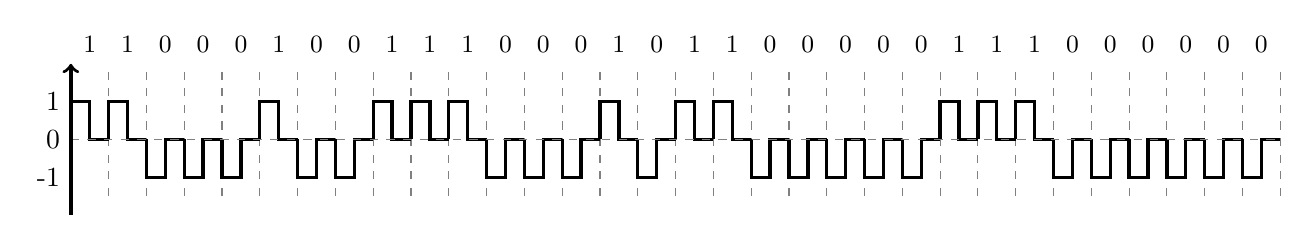
\begin{tikzpicture}[scale=0.48, very thick]
		\def\bits{1,1,0,0,0,1,0,0,1,1,1,0,0,0,1,0,1,1,0,0,0,0,0,1,1,1,0,0,0,0,0,0}

		\gdef\y{1}
		\foreach \b [count=\x from 0] in \bits {
			\draw[dashed, gray, thin] (\x+1,-1.5) -- (\x+1,2);
			\node at (\x+0.5, 2.5) {\small \b};
			\ifnum\b=1
				\ifnum\y=1
					\draw (\x,1) -- (\x+0.5,1) -- (\x+0.5,0) -- (\x+1,0);
					\xdef\y{0}
				\else
					\draw (\x,0) -- (\x,1) -- (\x+0.5,1) -- (\x+0.5,0) -- (\x+1,0);
					\xdef\y{0}
				\fi
			\else
				\draw (\x,0) -- (\x,-1) -- (\x+0.5,-1) -- (\x+0.5,0) -- (\x+1,0);
				\xdef\y{0}
			\fi
		}

		\draw[dashed, gray, thin] (0,0) -- (32,0);
		\draw[->] (0,-2) -- (0,2);

		\node[left] at (0,0) {0};
		\node[left] at (0,1) {1};
		\node[left] at (0,-1) {-1};
	\end{tikzpicture}
	\caption{RZ-кодирование исходного сообщения}
\end{figure}

\begin{figure}[H]
	\centering
	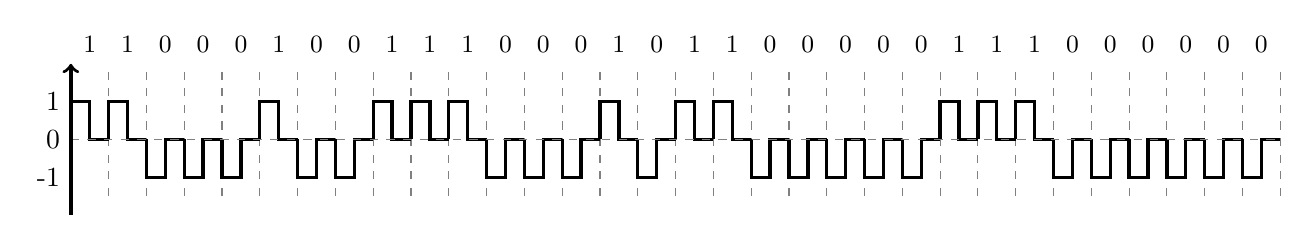
\begin{tikzpicture}[scale=0.48, very thick]
		\def\bits{1,1,0,0,0,1,0,0,1,1,1,0,0,0,1,0,1,1,0,0,0,0,0,1,1,1,0,0,0,0,0,0}

		\gdef\y{1}
		\foreach \b [count=\x from 0] in \bits {
			\draw[dashed, gray, thin] (\x+1,-1.5) -- (\x+1,2);
			\node at (\x+0.5, 2.5) {\small \b};
			\ifnum\b=1
				\ifnum\y=1
					\draw (\x,1) -- (\x+0.5,1) -- (\x+0.5,0) -- (\x+1,0);
					\xdef\y{0}
				\else
					\draw (\x,0) -- (\x,1) -- (\x+0.5,1) -- (\x+0.5,0) -- (\x+1,0);
					\xdef\y{0}
				\fi
			\else
				\draw (\x,0) -- (\x,-1) -- (\x+0.5,-1) -- (\x+0.5,0) -- (\x+1,0);
				\xdef\y{0}
			\fi
		}

		\draw[dashed, gray, thin] (0,0) -- (32,0);
		\draw[->] (0,-2) -- (0,2);

		\node[left] at (0,0) {0};
		\node[left] at (0,1) {1};
		\node[left] at (0,-1) {-1};
	\end{tikzpicture}
	\caption{RZ-кодирование исходного сообщения}
\end{figure}


% -----------------------------------------------------

\subsection{Потенциальный код с инверсий при 1 (NRZI)}
\begin{figure}[H]
	\centering
	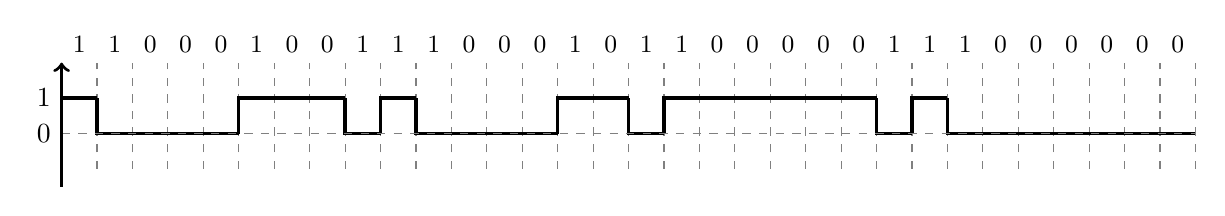
\begin{tikzpicture}[scale=0.45, very thick]
		\def\bits{1,1,0,0,0,1,0,0,1,1,1,0,0,0,1,0,1,1,0,0,0,0,0,1,1,1,0,0,0,0,0,0}

		\gdef\y{0}
		\foreach \b [count=\x from 0] in \bits {
			\draw[dashed, gray, thin] (\x+1,-1) -- (\x+1,2);
			\node at (\x+0.5, 2.5) {\small \b};
			\ifnum\b=1
				\ifnum\y=1
					\draw (\x,1) -- (\x,0) -- (\x+1,0);
					\xdef\y{0}
				\else
					\draw (\x,0) -- (\x,1) -- (\x+1,1);
					\xdef\y{1}
				\fi
			\else
				\draw (\x,\y) -- (\x+1,\y);
			\fi
		}

		\draw[dashed, gray, thin] (0,0) -- (32,0);
		\draw[->] (0,-1.5) -- (0,2);

		\node[left] at (0,0) {0};
		\node[left] at (0,1) {1};
	\end{tikzpicture}
	\caption{NRZI-кодирование исходного сообщения}
\end{figure}

\begin{figure}[H]
	\centering
	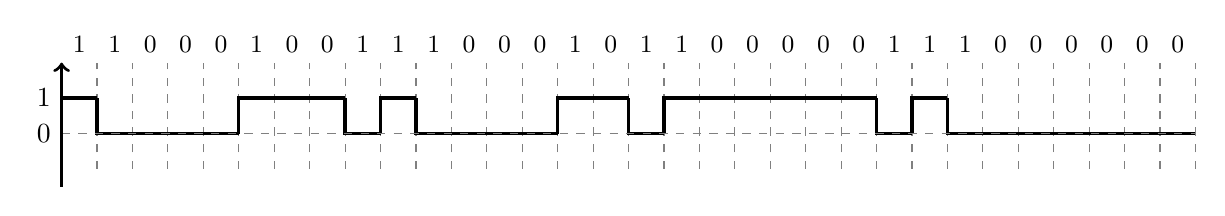
\begin{tikzpicture}[scale=0.45, very thick]
		\def\bits{1,1,0,0,0,1,0,0,1,1,1,0,0,0,1,0,1,1,0,0,0,0,0,1,1,1,0,0,0,0,0,0}

		\gdef\y{0}
		\foreach \b [count=\x from 0] in \bits {
			\draw[dashed, gray, thin] (\x+1,-1) -- (\x+1,2);
			\node at (\x+0.5, 2.5) {\small \b};
			\ifnum\b=1
				\ifnum\y=1
					\draw (\x,1) -- (\x,0) -- (\x+1,0);
					\xdef\y{0}
				\else
					\draw (\x,0) -- (\x,1) -- (\x+1,1);
					\xdef\y{1}
				\fi
			\else
				\draw (\x,\y) -- (\x+1,\y);
			\fi
		}

		\draw[dashed, gray, thin] (0,0) -- (32,0);
		\draw[->] (0,-1.5) -- (0,2);

		\node[left] at (0,0) {0};
		\node[left] at (0,1) {1};
	\end{tikzpicture}
	\caption{NRZI-кодирование исходного сообщения}
\end{figure}


% -----------------------------------------------------

\subsection{Манчестерский код}
\begin{figure}[H]
	\centering
	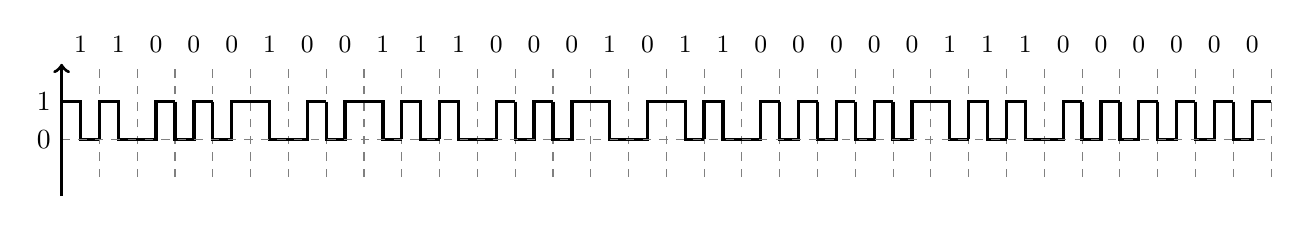
\begin{tikzpicture}[scale=0.48, very thick]
		\def\bits{1,1,0,0,0,1,0,0,1,1,1,0,0,0,1,0,1,1,0,0,0,0,0,1,1,1,0,0,0,0,0,0}

		\gdef\y{1}
		\foreach \b [count=\x from 0] in \bits {
			\draw[dashed, gray, thin] (\x+1,-1) -- (\x+1,2);
			\node at (\x+0.5, 2.5) {\small \b};
			\ifnum\b=1
				\ifnum\y=1
					\draw (\x,1) -- (\x+0.5,1) -- (\x+0.5,0) -- (\x+1,0);
					\xdef\y{0}
				\else
					\draw (\x,0) -- (\x,1) -- (\x+0.5,1) -- (\x+0.5,0) -- (\x+1,0);
					\xdef\y{0}
				\fi
			\else
				\ifnum\y=1
					\draw (\x,1) -- (\x,0) -- (\x+0.5,0) -- (\x+0.5,1) -- (\x+1,1);
					\xdef\y{1}
				\else
					\draw (\x,0) -- (\x+0.5,0) -- (\x+0.5,1) -- (\x+1,1);
					\xdef\y{1}
				\fi
			\fi
		}

		\draw[dashed, gray, thin] (0,0) -- (32,0);
		\draw[->] (0,-1.5) -- (0,2);

		\node[left] at (0,0) {0};
		\node[left] at (0,1) {1};
	\end{tikzpicture}
	\caption{Манчестерское кодирование исходного сообщения}
\end{figure}

\begin{figure}[H]
	\centering
	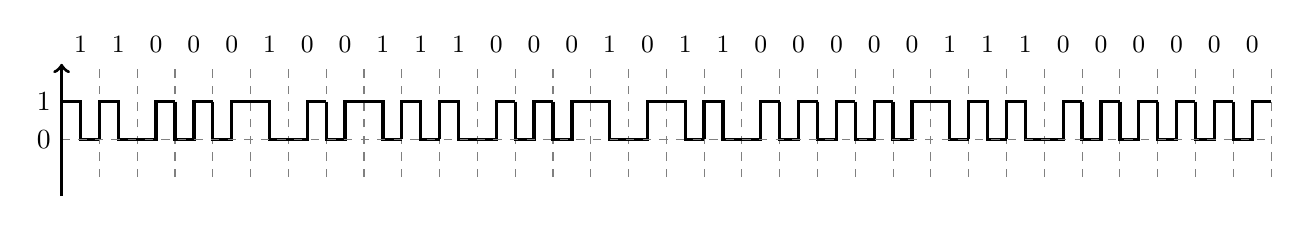
\begin{tikzpicture}[scale=0.48, very thick]
		\def\bits{1,1,0,0,0,1,0,0,1,1,1,0,0,0,1,0,1,1,0,0,0,0,0,1,1,1,0,0,0,0,0,0}

		\gdef\y{1}
		\foreach \b [count=\x from 0] in \bits {
			\draw[dashed, gray, thin] (\x+1,-1) -- (\x+1,2);
			\node at (\x+0.5, 2.5) {\small \b};
			\ifnum\b=1
				\ifnum\y=1
					\draw (\x,1) -- (\x+0.5,1) -- (\x+0.5,0) -- (\x+1,0);
					\xdef\y{0}
				\else
					\draw (\x,0) -- (\x,1) -- (\x+0.5,1) -- (\x+0.5,0) -- (\x+1,0);
					\xdef\y{0}
				\fi
			\else
				\ifnum\y=1
					\draw (\x,1) -- (\x,0) -- (\x+0.5,0) -- (\x+0.5,1) -- (\x+1,1);
					\xdef\y{1}
				\else
					\draw (\x,0) -- (\x+0.5,0) -- (\x+0.5,1) -- (\x+1,1);
					\xdef\y{1}
				\fi
			\fi
		}

		\draw[dashed, gray, thin] (0,0) -- (32,0);
		\draw[->] (0,-1.5) -- (0,2);

		\node[left] at (0,0) {0};
		\node[left] at (0,1) {1};
	\end{tikzpicture}
	\caption{Манчестерское кодирование исходного сообщения}
\end{figure}


% -----------------------------------------------------

\subsection{Дифференциальный манчестерский код}
\begin{figure}[H]
	\centering
	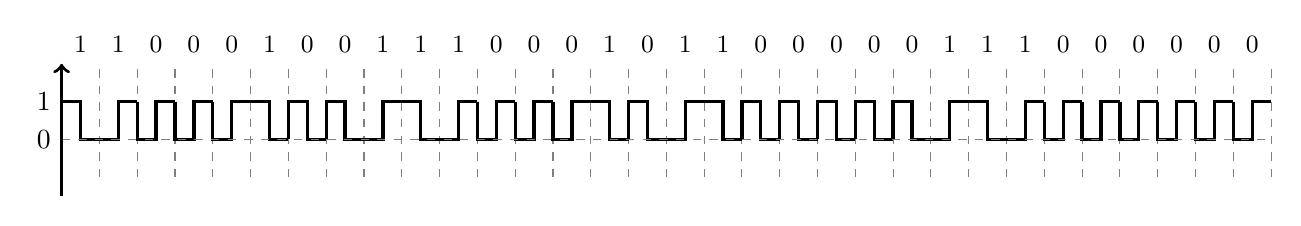
\begin{tikzpicture}[scale=0.48, very thick]
		\def\bits{1,1,0,0,0,1,0,0,1,1,1,0,0,0,1,0,1,1,0,0,0,0,0,1,1,1,0,0,0,0,0,0}

		\gdef\y{1}
		\foreach \b [count=\x from 0] in \bits {
			\draw[dashed, gray, thin] (\x+1,-1) -- (\x+1,2);
			\node at (\x+0.5, 2.5) {\small \b};
			\ifnum\b=0
				\ifnum\y=1
					\draw (\x,1) -- (\x,0) -- (\x+0.5,0) -- (\x+0.5,1) -- (\x+1,1);
					\xdef\y{1}
				\else
					\draw (\x,0) -- (\x,1) -- (\x+0.5,1) -- (\x+0.5,0) -- (\x+1,0);
					\xdef\y{0}
				\fi
			\else
				\ifnum\y=1
					\draw (\x,1) -- (\x+0.5,1) -- (\x+0.5,0) -- (\x+1,0);
					\xdef\y{0}
				\else
					\draw (\x,0) -- (\x+0.5,0) -- (\x+0.5,1) -- (\x+1,1);
					\xdef\y{1}
				\fi
			\fi
		}

		\draw[dashed, gray, thin] (0,0) -- (32,0);
		\draw[->] (0,-1.5) -- (0,2);

		\node[left] at (0,0) {0};
		\node[left] at (0,1) {1};
	\end{tikzpicture}
	\caption{Манчестерское дифференциальное кодирование исходного сообщения}
\end{figure}

\begin{figure}[H]
	\centering
	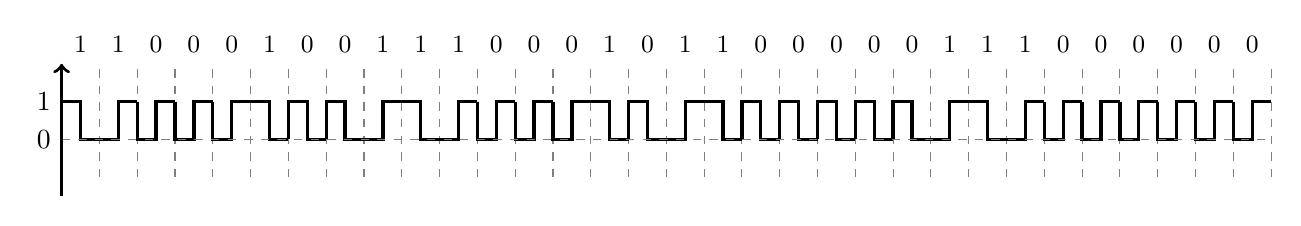
\begin{tikzpicture}[scale=0.48, very thick]
		\def\bits{1,1,0,0,0,1,0,0,1,1,1,0,0,0,1,0,1,1,0,0,0,0,0,1,1,1,0,0,0,0,0,0}

		\gdef\y{1}
		\foreach \b [count=\x from 0] in \bits {
			\draw[dashed, gray, thin] (\x+1,-1) -- (\x+1,2);
			\node at (\x+0.5, 2.5) {\small \b};
			\ifnum\b=0
				\ifnum\y=1
					\draw (\x,1) -- (\x,0) -- (\x+0.5,0) -- (\x+0.5,1) -- (\x+1,1);
					\xdef\y{1}
				\else
					\draw (\x,0) -- (\x,1) -- (\x+0.5,1) -- (\x+0.5,0) -- (\x+1,0);
					\xdef\y{0}
				\fi
			\else
				\ifnum\y=1
					\draw (\x,1) -- (\x+0.5,1) -- (\x+0.5,0) -- (\x+1,0);
					\xdef\y{0}
				\else
					\draw (\x,0) -- (\x+0.5,0) -- (\x+0.5,1) -- (\x+1,1);
					\xdef\y{1}
				\fi
			\fi
		}

		\draw[dashed, gray, thin] (0,0) -- (32,0);
		\draw[->] (0,-1.5) -- (0,2);

		\node[left] at (0,0) {0};
		\node[left] at (0,1) {1};
	\end{tikzpicture}
	\caption{Манчестерское дифференциальное кодирование исходного сообщения}
\end{figure}


% -----------------------------------------------------
%
% \subsection{PAM-5}
% \begin{figure}[H]
	\centering
	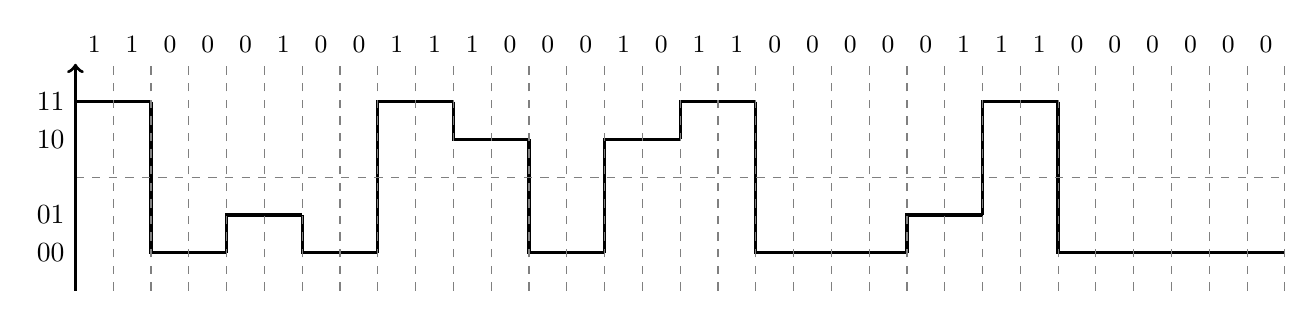
\begin{tikzpicture}[scale=0.48, very thick]
		\def\bits{1,1,0,0,0,1,0,0,1,1,1,0,0,0,1,0,1,1,0,0,0,0,0,1,1,1,0,0,0,0,0,0}
		\def\bbits{11,00,01,00,11,10,00,10,11,00,00,01,11,00,00,00}

		\gdef\y{2}
		\foreach \b [count=\x from 0] in \bbits {
			\ifnum\b=11
				\draw (\x*2,\y) -- (\x*2,2) -- (\x*2+2,2);
				\xdef\y{2}
			\fi

			\ifnum\b=10
				\draw (\x*2,\y) -- (\x*2,1) -- (\x*2+2,1);
				\xdef\y{1}
			\fi

			\ifnum\b=01
				\draw (\x*2,\y) -- (\x*2,-1) -- (\x*2+2,-1);
				\xdef\y{-1}
			\fi

			\ifnum\b=00
				\draw (\x*2,\y) -- (\x*2,-2) -- (\x*2+2,-2);
				\xdef\y{-2}
			\fi
		}

		\foreach \b [count=\x from 0] in \bits {
			\draw[dashed, gray, thin] (\x+1,-3) -- (\x+1,3);
			\node at (\x+0.5, 3.5) {\small \b};
		}

		\draw[dashed, gray, thin] (0,0) -- (32,0);
		\draw[->] (0,-3) -- (0,3);

		\node[left] at (0,2) {11};
		\node[left] at (0,1) {10};
		\node[left] at (0,0) {};
		\node[left] at (0,-1) {01};
		\node[left] at (0,-2) {00};
	\end{tikzpicture}
	\caption{PAM-5-кодирование исходного сообщения}
\end{figure}

% \begin{figure}[H]
	\centering
	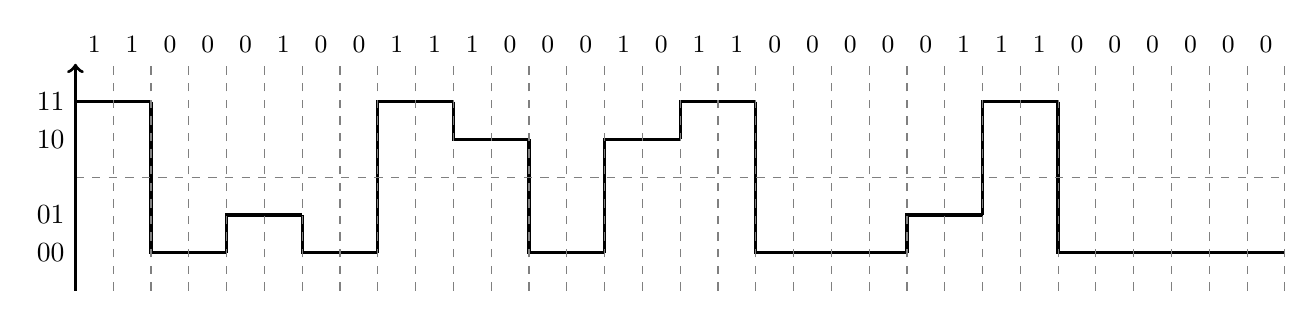
\begin{tikzpicture}[scale=0.48, very thick]
		\def\bits{1,1,0,0,0,1,0,0,1,1,1,0,0,0,1,0,1,1,0,0,0,0,0,1,1,1,0,0,0,0,0,0}
		\def\bbits{11,00,01,00,11,10,00,10,11,00,00,01,11,00,00,00}

		\gdef\y{2}
		\foreach \b [count=\x from 0] in \bbits {
			\ifnum\b=11
				\draw (\x*2,\y) -- (\x*2,2) -- (\x*2+2,2);
				\xdef\y{2}
			\fi

			\ifnum\b=10
				\draw (\x*2,\y) -- (\x*2,1) -- (\x*2+2,1);
				\xdef\y{1}
			\fi

			\ifnum\b=01
				\draw (\x*2,\y) -- (\x*2,-1) -- (\x*2+2,-1);
				\xdef\y{-1}
			\fi

			\ifnum\b=00
				\draw (\x*2,\y) -- (\x*2,-2) -- (\x*2+2,-2);
				\xdef\y{-2}
			\fi
		}

		\foreach \b [count=\x from 0] in \bits {
			\draw[dashed, gray, thin] (\x+1,-3) -- (\x+1,3);
			\node at (\x+0.5, 3.5) {\small \b};
		}

		\draw[dashed, gray, thin] (0,0) -- (32,0);
		\draw[->] (0,-3) -- (0,3);

		\node[left] at (0,2) {11};
		\node[left] at (0,1) {10};
		\node[left] at (0,0) {};
		\node[left] at (0,-1) {01};
		\node[left] at (0,-2) {00};
	\end{tikzpicture}
	\caption{PAM-5-кодирование исходного сообщения}
\end{figure}

